\part{Primeros pasos con MongoDB} 
\chapter{Conociendo MongoDB}

\section{MongoDB}

MongoDB\footnote{MongoDB - http://www.mongodb.org/} es un sistema de bases de datos no relacionales, multiplataforma e inspirada en el tipo de bases de datos documental y clave/valor, su nombre proviene del t\'ermino en ingl\'es "hu\textbf{mongo}us". Est\'a liberada bajo licencia de software libre, espec\'ificamente GNU AGPL 3.0\footnote{AGPL - http://www.gnu.org/licenses/agpl-3.0.html}. MongoDB usa el formato BSON (JSON Compilado) para guardar la informaci\'on, dando la libertad de manejar un esquema libre. Este motor de bases de datos es uno de los m\'as conocidos y usados, pudiendolo comparar en popularidad con MySQL en el caso de las bases de datos relacionales.

El desarrollo de MongoDB comenz\'o en el a\~no 2007 por la empresa 10gen\footnote{10gen - http://www.mongodb.com/}, publicando una version final en el 2009. Para la fecha que es escrito este libro, MongoDB se encuentra en la versi\'on 2.4.8.

\section{T\'erminos b\'asicos entorno a MongoDB}

\subsection{JSON - JavaScript Object Notation}

JSON es formato compacto de representacion de objetos. Las especificaciones las public\'o Douglas Crockford en el documento RFC 4627\footnote{RFC 4627 - http://www.ietf.org/rfc/rfc4627.txt}. JSON es un formato independiente del lenguaje, aunque su uso extendido hasta hace poco era en el lenguaje Javascipt. Actualmente se usa JSON en gran cantidades de sistemas para intercambiar informaci\'ion por su simplicidad en comparaci\'on con XML.

Este formato soporta gran cantidad de tipos de datos, lo que lo hace atractivo para un uso generalizado, y cada vez m\'as lenguajes de programaci\'on dan soporte a este formato. El ejemplo del cap\'itulo anterior, donde se mostraba un "documento", no es m\'as que JSON.

\subsection{Documento}

Un documento es un conjuto de datos estructurados (mas no con un esquema estricto), que contiene pares clave/valor, y se usa BSON (JSON Binario) como formato para almacenar los documentos. Un documento puede ser comparado con una fila o registro en una base de datos relacional.

\subsection{Colecci\'on}

Es un conjunto de documentos, similar a una tabla en las bases de datos relacionales.

\section{Instalando MongoDB}

\subsection{Instalaci\'on en Linux desde la fuente}

Existen distintas formas de instalar MongoDB en Linux, una de ellas, y la menos recomendable es compilar el c\'odigo fuente que pueden descargar desde: http://www.mongodb.org/downloads. Tambi\'en se puede descargar los binarios, descomprimirlos y usarlos.

\subsection{Instalaci\'on en Linux desde los repositorios}

Los sistemas Linux a diferencia de otros SO, manejo sus software en repositorios, que no es m\'as que un sitio centralizado donde se almacenan todos los software disponible para una distribuci\'on de Linux.

\subsection*{Instalaci\'on en Fedora Linux, Red Hat Linux Enterprise y Derivados}

Para instalar MongoDB en alguna de estras distribuciones, se debe hacer uso del gestor de paquetes yum y ejecutar el siguiente comando:

\begin{lstlisting}
    yum install mongodb mongodb-server
\end{lstlisting}

\begin{itemize}
    \item \textit{\textbf{mongodb}}: Contiene todos los paquetes ``cliente'', como es el caso del cliente \textbf{mongo}, la herramienta para respaldos en binarios de bases de datos \textbf{mongodump}, \textbf{mongorestore} para recuperar respaldos en binario, \textbf{mongoexport} y \textbf{mongoimport} que realizan una acc\'ion similar a mongodump y mongorestore, pero usan formato JSON o CSV.
    \item \textit{\textbf{mongodb-server}}: Contiene todos los paquetes para hacer funcionar el servidor, como el demonio \textbf{mongod}.
\end{itemize}

mongodb y mongodb-server se pueden instalar independientemente. ?`Cu\'ando hacer eso? Un caso muy representativo es cuando se desea colocar en producci\'on la base de datos. Se recomienda solo instalar los paquetes de servicio mongodb-server y el cliente en otra m\'aquina.

Para iniciar/reiniciar o apagar el demonio de MongoDB en \textbf{Fedora} se utiliza el siguiente comando:

\begin{lstlisting}
    systemctl start|restart|stop mongod.service
\end{lstlisting}

En el caso de \textbf{Red Hat Enterprise Linux 6} o derivados:

\begin{lstlisting}
    service mongod start|restart|stop
\end{lstlisting}

Para activar el inicio de MongoDB en el arranque del sistema debe ejecutar segun sea el caso lo siguiente:

\textbf{Fedora}

\begin{lstlisting}
    systemctl enable mongod.service
\end{lstlisting}

\textbf{Red Hat Enterprise Linux 6} o derivados:

\begin{lstlisting}
    chkconfig mongod on
\end{lstlisting}

\subsection*{Instalaci\'on en Debian}

En el caso de Debian, en un solo paquete se encuentra la distribuci\'on completa de MongoDB y para instalarlo se utiliza el gestor de paquetes apt-get:

\begin{lstlisting}
    apt-get install mongodb
\end{lstlisting}

\subsection*{Instalaci\'on en ArchLinux}

Haciendo uso del gestor de paquetes pacman:

\begin{lstlisting}
    pacman -S mongodb
\end{lstlisting}

\subsection{Instalaci\'on en Mac OS X}

\subsection*{Instalaci\'on Manual}

Puede descargar la \'ultima versi\'on disponible de MongoDB para Mac OS X usando cURL\footnote{cURL es una herramienta para usar en un intérprete de comandos para transferir archivos con sintaxis URL}, descomprimirlo y colocarlo en una carpeta a conveniencia.

\begin{lstlisting}
    curl -O http://downloads.mongodb.org/osx/mongodb-osx-x86_64-XXX.tgz
\end{lstlisting}

Siendo XXX, la versi\'on disponible. Ahora se descomprime el archivo usando la herramienta tar.

\begin{lstlisting}
    tar -zxvf mongodb-osx-x86_64-XXX.tgz
\end{lstlisting}

Con todos los archivos de MongoDB en su Mac OS X, solo debe ingresar a la carpeta resultante y ejecutar el demonio \textbf{mongod}.

\subsection*{Usando Homebrew}

\begin{lstlisting}
    brew update
    brew install mongodb
\end{lstlisting}

\section{La consola interactiva de MongoDB}

Ya con la previa instalaci\'on de MongoDB y sus herramientas, podemos acceder a su consola interactiva y realizar nuestras primeras interacciones con MongoDB.

\begin{figure}[!ht]
    \centering
    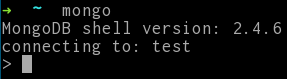
\includegraphics[scale=1]{img/mongodb_consola} 
    \caption[Consola de MongoDB]{Consola de MongoDB.}
\end{figure}

Al iniciar la consola se conecta autom\'aticamente a la base de datos \textit{\textbf{"test"}}, y apartir de all\'i podemos realizar consultas sobre esa base de datos. La consola es importante para administrar MongoDB, puede parecer desafiante para los que no est\'an acostumbrado a usar herramientas en c\'onsola, pero la gente de 10gen pens\'o en eso y agreg\'o comandos f\'aciles de recordar.

\subsection{Ayuda en la consola interactiva}

Para acceder a la ayuda de MongoDB en la consola, se utiliza el comando \textit{\textbf{help()}}.

\begin{lstlisting}
    > help
	db.help()                    help on db methods
	db.mycoll.help()             help on collection methods
	sh.help()                    sharding helpers
	rs.help()                    replica set helpers
	help admin                   administrative help
	help connect                 connecting to a db help
	help keys                    key shortcuts
	help misc                    misc things to know
	help mr                      mapreduce

	show dbs                     show database names
	show collections             show collections in current database
	show users                   show users in current database
	show profile                 show most recent system.profile entries with time >= 1ms
	show logs                    show the accessible logger names
	show log [name]              prints out the last segment of log in memory, 'global' is default
	use <db_name>                set current database
	db.foo.find()                list objects in collection foo
	db.foo.find( { a : 1 } )     list objects in foo where a == 1
	it                           result of the last line evaluated; use to further iterate
	DBQuery.shellBatchSize = x   set default number of items to display on shell
	exit                         quit the mongo shell
\end{lstlisting}

\section{Conectando a una base de datos}

La conexi\'on a bases de datos desde la consola o a trav\'es de alg\'un lenguaje es muy sencillo; a\'un as\'i en MongoDB NO se crean las bases de datos antes de usarla. En bases de datos relacionales, se debe crear toda una estructura inicial para poder almacenar informaci\'on, al menos se debe tener una base de datos con una tabla, eso en MongoDB no se hace. Para crear una base de datos se debe seleccionar, luego almacenar un documento creando una colecci\'on de documentos.

\subsection{Seleccionando la base de datos}

Antes de seleccionar una base de datos, uno tiene la opci\'on de ver el listado de bases de datos que existen en el sistema, con el comando \textit{\textbf{show dbs}}.

\begin{lstlisting}
    > show dbs
    admin	0.203125GB
    fudcon	0.453125GB
    irianas_server	0.203125GB
    irianas_web	0.203125GB
    local	0.078125GB
    mongoengine	0.203125GB
    mongoenginetest	0.203125GB
    mongoenginetest2	0.203125GB
    mongoenginetest4	0.203125GB
    test_files	0.203125GB
\end{lstlisting}

La salida nos muestra el nombre y el tama\~no de la base de datos, es importante mencionar que MongoDB al crear el primer documento reserva espacio en disco.

Luego de saber la lista de bases de datos existente, debo seleccionar una, no es obligatorio que est\'e en la lista, sencillamente haciendo uso del comando \textit{\textbf{use basededatos}}, se selecciona y podemos trabajar con la base de datos existente u operar para crear una nueva.

\begin{lstlisting}
    > use libromongodb
    switched to db libromongodb
\end{lstlisting}

Para confirmar la selecci\'on de la base de datos "libromongodb" en la sesi\'on, se verifica el valor del objecto \textit{\textbf{"db"}}.

\begin{lstlisting}
    > db
    libromongodb
\end{lstlisting}

\section{Nuestro primer documento}

Lleg\'o la hora de crear una base de datos y una colecci\'on, y eso se har\'a almacenando un documento usando el objeto \textit{\textbf{db}}, previa ejecuci\'on del comando \textit{\textbf{use}}. \textbf{Un documento puede tener en teor\'ia un m\'aximo de hasta 16MB de informaci\'on}. 

Aprovechando el ejemplo del primer cap\'itulo, para por fin almacenarlo en MongoDB y consultarlo. Una de las cosas que hay que tener en cuenta usando la consola interactiva, es usar variables para crear o modificar documentos, de esta manera podemos evitar accidentes con una mala manipulaci\'on directa de la base de datos.

Para almacenar un documento debemos ejecutar el m\'etodo \textit{\textbf{.insert()}} del objeto db, especificando el nombre de la colecci\'on (la colecci\'on se crea de manera din\'amica como la base de datos). Ejemplo:

\begin{lstlisting}
    > documento = {
    ...     _id: 1,
    ...     nombre: "MongoDB",
    ...     url: "http://www.mongodb.org",
    ...     tipo: "Documental"
    ...     }
    {
    	"_id" : 1,
    	"nombre" : "MongoDB",
    	"url" : "http://www.mongodb.org",
    	"tipo" : "Documental"
    }
    > db.nueva_coleccion.insert(documento)
\end{lstlisting}

De esta manera tenemos nuestra primera colecci\'on y nuestro primer documento, para confirmar esto, podemos ejecutar tanto el comando \textit{\textbf{show collections}} como el m\'etodo \textit{\textbf{.find()}}.

\begin{lstlisting}
    > show collections
    nueva_coleccion
    system.indexes
\end{lstlisting}

system.indexes es una colecci\'on que usa MongoDB para almacenar los \'indices de la colecci\'on. Por defecto \textit{\_id} es un \'indice.

\begin{lstlisting}
    > db.nueva_coleccion.find()
    { 
      "_id" : 1,
      "nombre" : "MongoDB",
      "url" : "http://www.mongodb.org",
      "tipo" : "Documental" }
\end{lstlisting}

Con \textit{\textbf{.find()}} se puede comprobar que efectivamente se almacen\'o el documento en la colecci\'on \textit{nueva\_colecci\'on}.